\documentclass[aspectratio=169]{beamer}
% Spin-polarized DT neutron wall loading: theory (Schwartz 2025), methods,
% and an OpenMC verification. Teaching deck.
% Build:  pdflatex spf_talk.tex  (run twice for the table of contents)
\usetheme{Madrid}
\usecolortheme{whale}
\usepackage{amsmath,amssymb}
\usepackage{graphicx}
\usepackage{booktabs}
\usepackage{xcolor}
\graphicspath{{../figs/}}
\setbeamertemplate{navigation symbols}{}
\setbeamertemplate{caption}{\raggedright\insertcaption\par}
\newcommand{\Bhat}{\hat{B}}
\newcommand{\dOmega}{\,d\Omega}

\title[Spin-polarized fusion NWL]{Steering Fusion Neutrons}
\subtitle{Spin-polarized DT wall loading: theory (Schwartz 2025), methods, and an OpenMC verification}
\author[SPF source project]{[Your Name]}
\institute[]{Prepared as a learning deck \\ \small (companion to the \texttt{spf\_prototype} OpenMC source)}
\date{\today}

\begin{document}

\begin{frame}[plain]\titlepage\end{frame}

\begin{frame}{What you'll get from this deck}
  \begin{itemize}
    \item \alert{Part I --- Physics:} why spin-polarized fusion steers neutrons, and the cross section that does it.
    \item \alert{Part II --- Analytic wall load:} how Schwartz (2025) turns that into a fast, closed-form neutron wall load (NWL).
    \item \alert{Part III --- Our prototype:} a polarization-aware \emph{OpenMC} source and a tiered verification.
    \item \alert{Part IV --- Results:} sampler $\to$ independent analytic $\to$ full Monte-Carlo, plus engineering scalars.
    \item \alert{Part V --- Honest scope \& what's next.}
  \end{itemize}
  \vfill
  \footnotesize Primary reference: J.~A.~Schwartz, \emph{Analytic neutron wall loading from spin-polarized fusion in axisymmetric geometries}, arXiv:2507.11758 (2025).
\end{frame}

\begin{frame}{Outline}\tableofcontents\end{frame}

% ======================================================================
\section{Part I --- The physics of spin-polarized fusion}
% ======================================================================
\begin{frame}{Why polarize the fuel?}
  Align the nuclear spins of the D and T fuel \emph{before} they react. Two payoffs:
  \begin{itemize}
    \item \alert{Rate:} the fusion cross section can rise by up to \alert{50\%}.
    \item \alert{Direction:} neutrons (and alphas) are emitted \alert{anisotropically} --- preferentially along or across the magnetic field.
  \end{itemize}
  \vfill
  Engineering hook: \alert{aim neutrons away from fragile structures} (tokamak center stack, divertor; mirror end plugs; dipole flyer ring) and toward robust outer walls.
  \vfill
  \footnotesize The two effects are \emph{not} independent --- the spin mix that boosts rate is not the same as the one that best steers. Choosing the mix is a design trade-off.
\end{frame}

\begin{frame}{Spin states of the reactants}
  \begin{itemize}
    \item \alert{Deuteron} (spin 1): projection on $\Bhat$ can be $m=+1,0,-1$. Fractions $d_+,\,d_0,\,d_-$.
    \item \alert{Triton} (spin $\tfrac12$): projection $m=\pm\tfrac12$. Fractions $t_+,\,t_-$.
  \end{itemize}
  \vfill
  Six spin combinations $\to$ by symmetry about $\Bhat$ they collapse to \alert{three collision modes} $a,b,c$ (Schwartz Eq.~1):
  \[
    a = d_+ t_+ + d_- t_-, \qquad
    b = d_0\;(= d_0 t_+ + d_0 t_-), \qquad
    c = d_+ t_- + d_- t_+ .
  \]
  with $a+b+c=1$. \quad Unpolarized fuel: $a=b=c=\tfrac13$.
  \vfill
  \footnotesize $b$ is just the deuteron transverse ($m=0$) fraction. The three spin fractions give 3 knobs, but the emission depends on only \alert{2 degrees of freedom}.
\end{frame}

\begin{frame}{The differential cross section (Schwartz Eq.~2)}
  Let $\theta$ be the angle between the emitted neutron and the \alert{local field direction $\Bhat$}:
  \[
    \frac{d\sigma}{d\Omega}
    = \frac{\sigma_0}{2\pi}\left[\;
      \tfrac{3}{4}\,a\,\sin^2\theta
      \;+\;\Big(\tfrac{2}{3}b+\tfrac{1}{3}c\Big)\Big(\tfrac14+\tfrac34\cos^2\theta\Big)
    \;\right]
  \]
  $\sigma_0$ = cross section in the $S=\tfrac32$ combined-spin state.
  \vfill
  \begin{itemize}
    \item The $\sin^2\theta$ piece (weight $\propto a$): emission \alert{perpendicular} to $\Bhat$.
    \item The $\tfrac14+\tfrac34\cos^2\theta$ piece (weight $\propto \tfrac23 b+\tfrac13 c$): emission \alert{parallel} to $\Bhat$.
  \end{itemize}
  \vfill
  \footnotesize Everything that follows --- rate, directionality, wall load --- is a consequence of this one formula.
\end{frame}

\begin{frame}{Integrate over the sphere: the total rate factor $\eta$}
  Using $\displaystyle\int \sin^2\theta\dOmega=\frac{8\pi}{3}$ and $\displaystyle\int\Big(\tfrac14+\tfrac34\cos^2\theta\Big)\dOmega=2\pi$:
  \[
    \sigma_{\text{tot}} = \sigma_0\Big(a+\tfrac23 b+\tfrac13 c\Big)\equiv \sigma_0\,\eta .
  \]
  $\eta$ is the \alert{total-rate factor} (relative to $\sigma_0$). Corner values:
  \begin{center}\footnotesize
  \begin{tabular}{lccc}
    \toprule
    mode & $(a,b,c)$ & $\sigma_{\text{tot}}/\sigma_0=\eta$ & vs.\ unpolarized\\
    \midrule
    unpolarized & $(\tfrac13,\tfrac13,\tfrac13)$ & $2/3$ & --- \\
    \alert{A} & $(1,0,0)$ & $1$ & $+50\%$ \\
    \alert{B} & $(0,1,0)$ & $2/3$ & same \\
    \alert{C} & $(0,0,1)$ & $1/3$ & $-50\%$ \\
    \bottomrule
  \end{tabular}
  \end{center}
  \vfill
  \footnotesize Note: the unpolarized total is $2\sigma_0/3$, \emph{not} $\sigma_0$. The ``50\% enhancement'' is A's $\sigma_0$ relative to that $2\sigma_0/3$.
\end{frame}

\begin{frame}{The three pure modes --- shapes and a key correction}
  \begin{itemize}
    \item \alert{A mode} $(1,0,0)$: $\dfrac{d\sigma}{d\Omega}\propto\sin^2\theta$ --- vanishes along $\Bhat$, peaks \alert{perpendicular}. Highest rate.
    \item \alert{B mode} $(0,1,0)$: $\propto\tfrac14+\tfrac34\cos^2\theta$ --- peaks \alert{parallel} to $\Bhat$. Same total as unpolarized.
    \item \alert{C mode} $(0,0,1)$: \alert{same angular shape as B} ($\tfrac14+\tfrac34\cos^2\theta$); only the \emph{rate} differs (half the unpolarized rate).
  \end{itemize}
  \vfill
  \alert{Correction to a common mistake:} C is \alert{not} isotropic. Set $a=0$ in Eq.~2 --- the $b$ and $c$ terms carry the \emph{identical} $\theta$-dependence. So \alert{B and C share directionality}; they differ only in magnitude.
\end{frame}

\begin{frame}{Separating ``where'' from ``how many''}
  The birth-direction shape depends on only \alert{two effective weights}:
  \[
    w_\perp=\tfrac34 a \quad(\sin^2\theta\text{ piece}),\qquad
    w_\parallel=\tfrac23 b+\tfrac13 c\quad(\tfrac14+\tfrac34\cos^2\theta\text{ piece}).
  \]
  Unnormalized birth intensity about $\Bhat$:
  \[
    I(\theta)=w_\perp\sin^2\theta+w_\parallel\Big(\tfrac14+\tfrac34\cos^2\theta\Big),\qquad
    p(\theta,\varphi)=\frac{I(\theta)}{\int I\dOmega},\;\; \varphi\sim U[0,2\pi).
  \]
  \vfill
  \alert{Design takeaway:} the \emph{direction} pdf needs only $(w_\perp,w_\parallel)$; the \emph{total rate} $\eta$ is a separate scalar. Keeping these two concerns apart is the single most important modeling decision --- it mirrors how Schwartz separates angular factors from rate factors.
\end{frame}

\begin{frame}{Energy (for completeness)}
  \begin{itemize}
    \item Birth energy is \alert{decoupled} from the polarized angular distribution to leading order.
    \item For the analytic comparison: \alert{monoenergetic 14.1 MeV} (Schwartz drops the energy spread entirely).
    \item A physical option (not used in verification): a Ballabio-broadened Gaussian at ion temperature $T_i$ (width $\approx 177\sqrt{T_i[\text{keV}]}$ keV).
  \end{itemize}
  \vfill
  Energy is irrelevant to the \emph{angular}/geometric wall-load physics, so we set it aside.
\end{frame}

% ======================================================================
\section{Part II --- The analytic neutron wall load (Schwartz)}
% ======================================================================
\begin{frame}{What is ``neutron wall load'' (NWL)?}
  Following Lion, the NWL is the neutron current through a patch of first wall (Schwartz Eq.~3):
  \[
    Q^{\text{NWL}}(\mathbf r_w)=\frac{E_n}{4\pi}\int_{V_s} dV\;
      \Phi^{\text{src}}(\mathbf r_s)\;\Bhat_n\!\cdot\!\frac{\mathbf r_s-\mathbf r_w}{|\mathbf r_s-\mathbf r_w|^3}
  \]
  $E_n$ = energy/neutron, $\Phi^{\text{src}}$ = source density, $\hat n$ = wall normal.
  \vfill
  \begin{itemize}
    \item For an \alert{isotropic} source the $1/4\pi$ is a constant; for a \alert{polarized} source we insert the angular factor in $\cos\theta$ (angle to local $\Bhat$).
    \item \alert{Crucial:} this is a \alert{free-streaming, sightline} quantity --- \alert{no scattering}. It is a \emph{geometric} load, not a shielded dose, not a TBR.
  \end{itemize}
\end{frame}

\begin{frame}{Geometry: a filamentary ring source}
  Schwartz reduces the volume integral to a 1-D toroidal integral over a \alert{ring} of plasma at major radius $p$, height $z$:
  \begin{columns}[T]
    \begin{column}{0.58\linewidth}
      \begin{itemize}\small
        \item Source point $S=(p\cos\varphi,\,p\sin\varphi,\,z)$.
        \item Target $T$ on the wall (radius $u$ on the inboard side), normal $\hat n$.
        \item $\boldsymbol\Delta=S-T=(p\cos\varphi-u,\,p\sin\varphi,\,z)$,
        \item $|\boldsymbol\Delta|=\sqrt{p^2+u^2+z^2-2pu\cos\varphi}$.
        \item $\cos\nu=\dfrac{\boldsymbol\Delta\cdot\hat n}{|\boldsymbol\Delta|}=\dfrac{p\cos\varphi-u}{|\boldsymbol\Delta|}$ (inboard).
        \item Visible arc $\pm\varphi_i=\arccos(u/p)$.
      \end{itemize}
    \end{column}
    \begin{column}{0.42\linewidth}
      \footnotesize $\nu$ = angle between sightline and wall normal.\\[2pt]
      $\theta$ = angle between sightline and $\Bhat$.\\[2pt]
      The ring is integrated only over the arc \alert{visible} from the target.
    \end{column}
  \end{columns}
\end{frame}

\begin{frame}{The reduced intensity $g$}
  Per unit ring length (dropping $E_n/4\pi$), the wall load from one ring is
  \[
    g=\int_{-\varphi_m}^{\varphi_m} \frac{p\,\cos\nu}{|\boldsymbol\Delta|^2}\,f(\cos\theta)\,d\varphi,
  \]
  with the angular factor $f$:
  \[
    f=1\ (\text{iso}),\quad f=\sin^2\theta\ (\text{A}),\quad f=\tfrac14+\tfrac34\cos^2\theta\ (\text{B/C}).
  \]
  For a \alert{purely toroidal} field $\Bhat=(-\sin\varphi,\cos\varphi,0)$ one finds the compact result
  \[
    \cos\theta=\frac{u\sin\varphi}{|\boldsymbol\Delta|}\qquad(\text{Schwartz Eq.~7}).
  \]
  \vfill
  \footnotesize $1/|\boldsymbol\Delta|^2$ = inverse-square fall-off; $\cos\nu$ = projection onto the wall; $p\,d\varphi$ = ring line element.
\end{frame}

\begin{frame}{Closed form via elliptic integrals (Schwartz Eq.~5)}
  The integrals evaluate in terms of incomplete elliptic integrals $F(\varphi,m),E(\varphi,m)$. E.g.\ inboard, isotropic:
  \[\resizebox{\linewidth}{!}{$\displaystyle
    g_{RiI}=\frac{4p\sqrt{(p^2-u^2)(p^2-u^2+z^2)}}{q}
    -\frac{2p\,F(\varphi,m)}{u\sqrt{(p-u)^2+z^2}}
    +\frac{2p(p^2-u^2+z^2)\sqrt{(p-u)^2+z^2}}{q\,u}\,E(\varphi,m)
  $}\]
  \[
    q=p^4-2p^2(u^2-z^2)+(u^2+z^2)^2,\quad \varphi=\tfrac{\varphi_i}{2},\quad m=\frac{-4pu}{(p-u)^2+z^2}.
  \]
  \begin{itemize}
    \item Floor/ceiling and outboard walls: same structure, different normal and visibility limits (Schwartz \S3.3--3.4).
    \item \alert{Fully differentiable} $\Rightarrow$ usable inside a gradient-based design optimizer.
  \end{itemize}
\end{frame}

\begin{frame}{\texttt{anarr\'ima}: Schwartz's reference implementation}
  \begin{itemize}
    \item Open-source \texttt{python} package (PrincetonUniversity/\texttt{anarrima}), \alert{JAX}-based (auto-differentiable).
    \item Implements the closed forms: \texttt{g\_HI/g\_HA/g\_Hc/g\_HB} (horizontal-normal walls) and \texttt{g\_VI/...} (vertical), plus angled-field variants (\S3.2).
    \item Ships an \texttt{examples/square\_torus.py} that generates the paper's Figure~2.
  \end{itemize}
  \vfill
  \alert{We use it as the ``ground-truth'' analytic reference} --- and cross-check it with our own independent quadrature.
\end{frame}

\begin{frame}{Schwartz's headline example: square-cross-section torus}
  Circular plasma (parabolic $1-\rho^2$ profile), purely toroidal field, four flat walls. Holding \alert{total fusion rate constant}, compare directionality:
  \begin{center}\footnotesize
  \begin{tabular}{lcc}
    \toprule
    quantity & effect (paper text) \\
    \midrule
    isotropic: outboard vs inboard & outboard $\sim\!12\%$ hotter (pure geometry)\\
    A mode, inboard midplane & $+43\%$ \\
    A mode, outboard midplane & $-22\%$ \\
    B/C mode (mirror of A) & $-43\%$ inboard, $+22\%$ outboard \\
    \bottomrule
  \end{tabular}
  \end{center}
  \vfill
  \alert{Physics story:} B/C steers neutrons \alert{off the inboard center stack} toward the outboard wall --- attractive for spherical tokamaks where the center stack is precious.
\end{frame}

% ======================================================================
\section{Part III --- Our prototype: a polarization-aware OpenMC source}
% ======================================================================
\begin{frame}{Goal and method}
  \alert{Goal:} a self-contained, polarization-aware \emph{birth-direction sampler} for OpenMC --- validated against (i) the unpolarized isotropic limit and (ii) Schwartz's analytic results --- before any integration with a real plasma source.
  \vfill
  \alert{Working style (strict):}
  \begin{itemize}
    \item Hard-gate on correctness; \alert{strict tier ordering} (don't start tier $N{+}1$ until $N$ passes).
    \item Honest, non-cherry-picked diagnostics (report marginal/failed results plainly).
    \item Asserts for invariants; warnings only for user input.
  \end{itemize}
\end{frame}

\begin{frame}{The tiers}
  \begin{itemize}
    \item \alert{Tier 0 --- Environment:} build OpenMC, install, cross sections, verify the custom-source build recipe end-to-end.
    \item \alert{Tier 1 --- Sampler alone} (no transport): get the birth directions provably right.
    \item \alert{Tier 2a --- Independent analytic NWL:} reimplement Schwartz's integral; agree with \texttt{anarr\'ima}.
    \item \alert{Tier 2b --- Full Monte-Carlo:} run the compiled source through OpenMC; reproduce the analytic.
    \item \alert{Tier 3 --- Engineering artifacts:} peaking factors, current fractions, figures.
  \end{itemize}
\end{frame}

\begin{frame}{Sampler architecture (one source of truth)}
  \begin{itemize}
    \item \texttt{spf\_sampler.hpp} --- \alert{pure-math header}: $(a,b,c)\!\to\!(w_\perp,w_\parallel,\eta)$, the angular samplers, and the frame rotation. No OpenMC types $\Rightarrow$ testable standalone.
    \item \texttt{spf\_mirror.py} --- a \alert{Python mirror}, including a \emph{bit-exact} port of OpenMC's PCG \texttt{prn}.
    \item \texttt{polarized\_fusion\_source.cpp} --- a thin \texttt{openmc::Source} wrapper (the \texttt{.so}).
  \end{itemize}
  \vfill
  \alert{Why this split?} ``C++ vs Python on identical seeds'' becomes a transcription-bug catcher, and Tier 1 needs no \texttt{libopenmc}.
  \vfill
  \footnotesize Thread-safety: all state set in the constructor and \texttt{const} thereafter; randomness only via \texttt{openmc::prn(seed)} --- no data races.
\end{frame}

\begin{frame}{Method: stratified angular sampling}
  The mixture pdf is a blend of two shapes. Sample exactly by \alert{stratification}:
  \[
    P_\perp=\frac{W_\perp}{W_\perp+W_\parallel}=\frac{a}{\eta},
    \qquad W_\perp=w_\perp\!\int\!\sin^2\theta\dOmega,\;\; W_\parallel=w_\parallel\!\int\!\big(\tfrac14+\tfrac34\cos^2\theta\big)\dOmega.
  \]
  \begin{itemize}
    \item With prob.\ $P_\perp$ draw the $\sin^2\theta$ shape; else the $\tfrac14+\tfrac34\cos^2\theta$ shape.
    \item Then $\varphi\sim U[0,2\pi)$, and rotate into the lab frame.
  \end{itemize}
  \vfill
  \alert{Direction and rate are decoupled:} the same stratified split samples directions for \emph{any} $(a,b,c)$; the scalar $\eta$ rides separately on the source strength.
\end{frame}

\begin{frame}{Method: exact inverse-CDF for each shape}
  Work in $x=\cos\theta$ (so $d\Omega=d\varphi\,dx$):
  \begin{itemize}
    \item \alert{$\sin^2\theta$ shape:} $p(x)\propto 1-x^2$. Inverse-CDF solves the depressed cubic
      \[
        x^3-3x+(4u-2)=0,\qquad x=2\cos\!\Big(\tfrac13\arccos(1-2u)-\tfrac{2\pi}{3}\Big).
      \]
    \item \alert{$\tfrac14+\tfrac34\cos^2\theta$ shape:} $p(x)=\tfrac14+\tfrac34 x^2$. Inverse-CDF solves
      \[
        x^3+x+(2-4u)=0\quad(\text{single real root, Cardano}).
      \]
  \end{itemize}
  \vfill
  Both roots are endpoint-verified ($u\!=\!0\!\to\!x\!=\!-1$, $u\!=\!1\!\to\!x\!=\!+1$) and \alert{cross-checked against a rejection sampler} (two-sample KS).
  \vfill
  \footnotesize (The form in my notes, $x^3-3x+2(1-2u)=0$, is the same sampler under $u\!\to\!1-u$ --- equivalent, but we use the endpoint-verified version.)
\end{frame}

\begin{frame}{Method: local $\to$ global rotation (no gimbal trap)}
  Sample in a frame with $\hat z_{\text{loc}}\parallel\Bhat$, then rotate to lab. \alert{Avoid} building the basis from $\Bhat\times\hat z_{\text{world}}$ (degenerate when $\Bhat\parallel\hat z$). Instead:
  \begin{enumerate}
    \item pick reference axis $\mathbf r$ = whichever of $\hat x,\hat y,\hat z$ has the smallest $|\Bhat\cdot\hat e|$;
    \item $\hat x_{\text{loc}}=\text{normalize}(\mathbf r-(\mathbf r\!\cdot\!\Bhat)\Bhat)$, \;$\hat y_{\text{loc}}=\Bhat\times\hat x_{\text{loc}}$, \;$\hat z_{\text{loc}}=\Bhat$;
    \item $\mathbf u_{\text{global}} = x_{\text{loc}}\hat x_{\text{loc}}+y_{\text{loc}}\hat y_{\text{loc}}+z_{\text{loc}}\Bhat$.
  \end{enumerate}
  \vfill
  Robust for \alert{any} $\Bhat$ (including $\pm\hat z$); the result is asserted unit to $10^{-12}$.
\end{frame}

% ======================================================================
\section{Part IV --- Results}
% ======================================================================
\begin{frame}{Tier 1 --- the sampler is provably correct}
  All checks call the math directly (no transport). Highlights:
  \begin{itemize}
    \item \alert{Mode identities (sympy):} $\int d\sigma/d\Omega\dOmega=\sigma_0(a+\tfrac23 b+\tfrac13 c)$; corners $2/3,1,2/3,1/3$; B and C share shape.
    \item \alert{C++ vs Python parity:} max $|\Delta|=\mathbf{6\times10^{-16}}$ on identical seeds (RNG, both cubics, rotation all match).
    \item \alert{Per-mode $\cos\theta$:} $\chi^2/\text{dof}\approx 1$; A vanishes at $\cos\theta=\pm1$, B/C peak there, unpolarized is flat.
    \item \alert{Steering oracle} $\langle\cos^2\theta\rangle$: A $=1/5$, B/C $=7/15$, iso $=1/3$ --- all reproduced; rotation preserves isotropy; $\Bhat=\pm\hat z$ fine.
  \end{itemize}
\end{frame}

\begin{frame}{Tier 1 --- per-mode birth distribution vs analytic}
  \begin{center}
    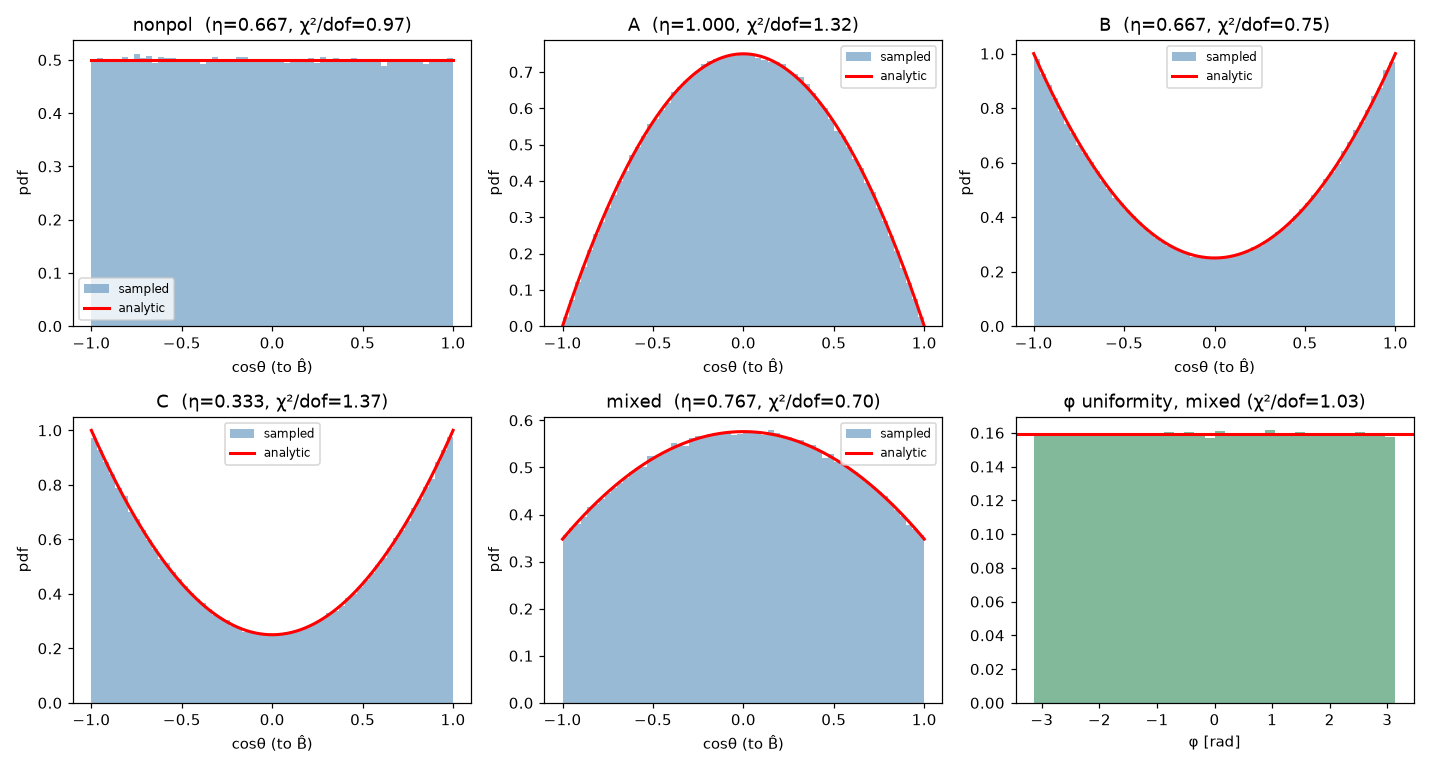
\includegraphics[width=0.76\linewidth]{tier1_costheta_per_mode.png}
  \end{center}
  \footnotesize Sampled $\cos\theta$ (bars) vs analytic pdf (red). Unpolarized flat; A $=\sin^2\theta$ dome (zero at $\pm1$); \alert{B and C the identical} $\tfrac14+\tfrac34\cos^2\theta$ U-shape; $\varphi$ uniform. Confirms B$\equiv$C.
\end{frame}

\begin{frame}{Tier 2a --- an independent analytic NWL}
  Three \alert{independent} engines for the single-ring reduced intensity $g$:
  \begin{enumerate}
    \item our vectorized \alert{Gauss--Legendre quadrature} of the $g$ integral;
    \item \alert{\texttt{anarr\'ima}} (Schwartz's closed forms);
    \item our own transcription of the \alert{Eq.~5} elliptic closed form.
  \end{enumerate}
  \vfill
  \begin{itemize}
    \item Single central ring: all three agree to $\mathbf{1.8\times10^{-15}}$ (all walls, all modes).
    \item Free internal identities hold exactly: $g_{\text{iso}}=g_A+g_{\cos^2}$ and $g_{\text{B/C}}=\tfrac14 g_{\text{iso}}+\tfrac34 g_{\cos^2}$.
    \item Parabolic plasma $=\sum$ rings weighted by $1-\rho^2$: quadrature vs \texttt{anarr\'ima} agree to $\mathbf{5\times10^{-8}}$ over all wall points.
  \end{itemize}
\end{frame}

\begin{frame}{Tier 2a --- reproducing Schwartz Figure 2}
  \begin{center}
    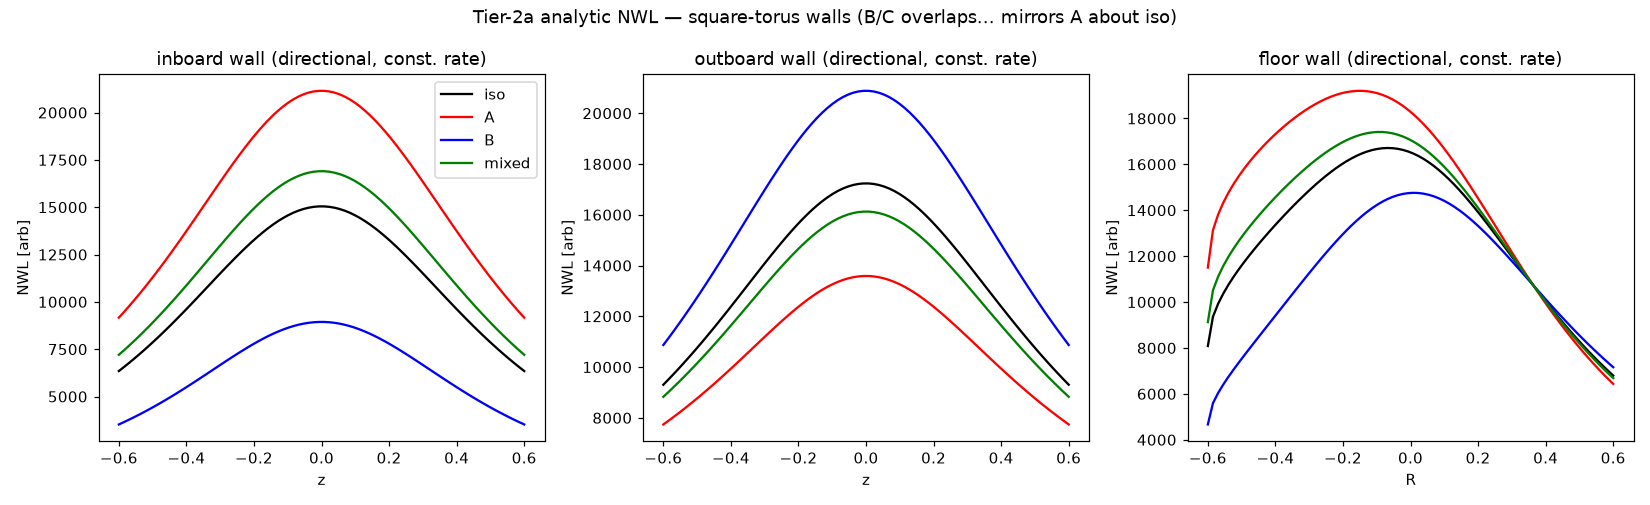
\includegraphics[width=0.86\linewidth]{tier2a_nwl_walls.png}
  \end{center}
  \footnotesize Constant-rate directional NWL on the three walls. A (red) loads the inboard, B/C (blue) the outboard; floor shows the cross-over. Scalar oracles: A $+40.6\%$ inboard, $-21.2\%$ outboard; iso outboard/inboard $+14.6\%$. \alert{These match \texttt{anarr\'ima}'s own example exactly} (paper text rounds to $43/22/12$).
\end{frame}

\begin{frame}{Tier 2a --- two findings to carry forward}
  \begin{itemize}
    \item \alert{iso $\ne$ C.} The normalized pattern of C is the \alert{mirror of B}, not isotropic (C is $-40.6\%$ at the center stack, like B). The valid cheap equivalence is \alert{B $\equiv$ C}, which holds exactly. (A spec that says ``iso $\equiv$ C'' is wrong.)
    \item \alert{Aspect ratio.} The paper \emph{text} says aspect ratio 2.5, but the figure-generating code uses \alert{2.0} ($R_0{=}1,a{=}0.5$, walls $u{=}0.4,w{=}1.6,z{=}\pm0.6$). We match the reference \emph{implementation}.
  \end{itemize}
\end{frame}

\begin{frame}{Tier 2b --- full Monte-Carlo in OpenMC}
  \begin{itemize}
    \item Compiled the source into a \texttt{.so} (\texttt{find\_package(OpenMC)} + \texttt{OpenMC::libopenmc}).
    \item Square-cross-section torus, \alert{near-void interior} $\Rightarrow$ free-streaming (Leakage $=1$; boundary-current conservation $=1.0000$).
    \item Tally: \alert{surface current} on a \texttt{CylindricalMesh} (\texttt{MeshSurfaceFilter}), $\ge 50$ poloidal bins per wall.
    \item Configs $\{$iso, A, B, C, mixed$\}$; compare \alert{directionality} (mode/iso, normalization-free) to the exact $D=\text{bracket}/\eta$.
  \end{itemize}
  \vfill
  \footnotesize Geometry identical to the analytic, so bins map 1:1.
\end{frame}

\begin{frame}{Tier 2b --- OpenMC reproduces the analytic}
  \begin{center}
    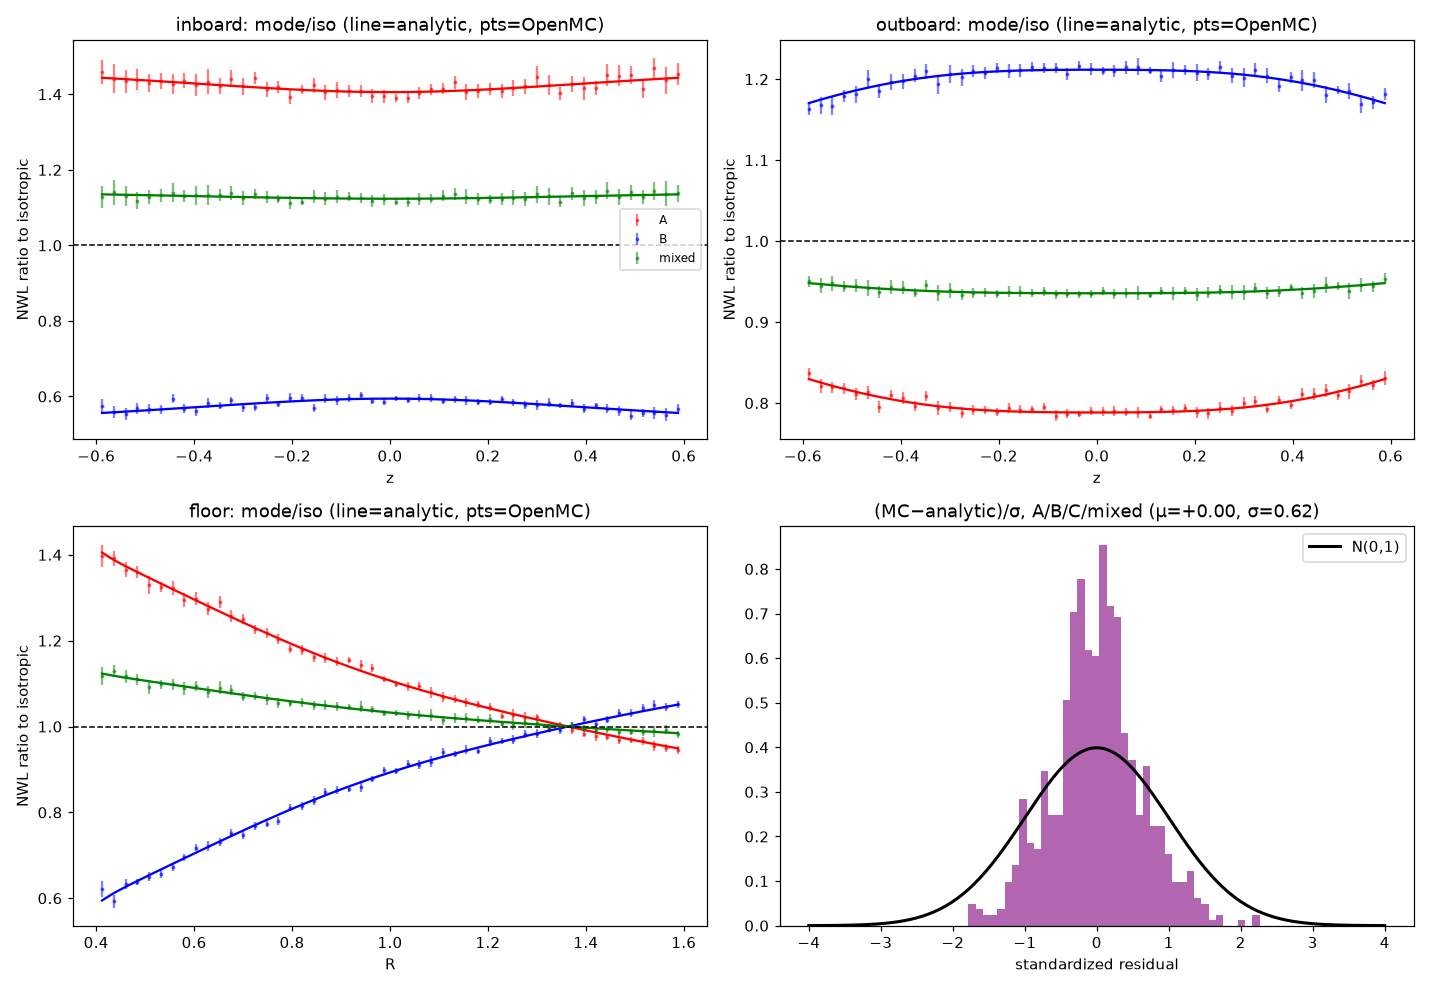
\includegraphics[width=0.60\linewidth]{tier2b_nwl_compare.png}
  \end{center}
  \footnotesize Points = OpenMC, lines = analytic. Residual $(\text{MC}-\text{analytic})/\sigma$: \alert{mean $\approx0$}, $\sigma\approx0.69$. MC oracles match the analytic (A $+39\%$ inboard, $-21\%$ outboard); \alert{B$\equiv$C} and \alert{linearity} ($\text{mixed}=0.5A{+}0.3B{+}0.2C$) hold.
\end{frame}

\begin{frame}{Tier 3 --- engineering scalars (the honest part)}
  Postprocessing the existing Tier-2b data (no new runs). Per mode, constant fusion rate:
  \begin{center}\footnotesize
  \begin{tabular}{lcccc}
    \toprule
    & iso & A & B/C \\
    \midrule
    inboard peak vs iso & --- & $+39.5\%$ & $-40.9\%$ \\
    outboard peak vs iso & --- & $-21.0\%$ & $+21.1\%$ \\
    inboard current fraction & $8.7\%$ & $12.3\%$ & $\mathbf{5.1\%}$ \\
    \alert{overall peaking factor} & $\mathbf{1.33}$ & $\mathbf{1.65}$ & $\mathbf{1.61}$ \\
    \bottomrule
  \end{tabular}
  \end{center}
  \vfill
  \alert{Counter-intuitive, but real:} in a \emph{fixed} geometry, polarization \alert{raises} the overall peaking factor (directional emission concentrates load; isotropic is the most uniform). B/C's benefit is the \alert{center-stack reduction} (inboard current $8.7\%\!\to\!5.1\%$), \alert{not} a lower peaking factor. Schwartz's peaking \emph{reduction} comes from then re-shaping the wall --- not modeled here.
\end{frame}

\begin{frame}{Tier 3 --- the picture for a one-glance audience}
  \begin{center}
    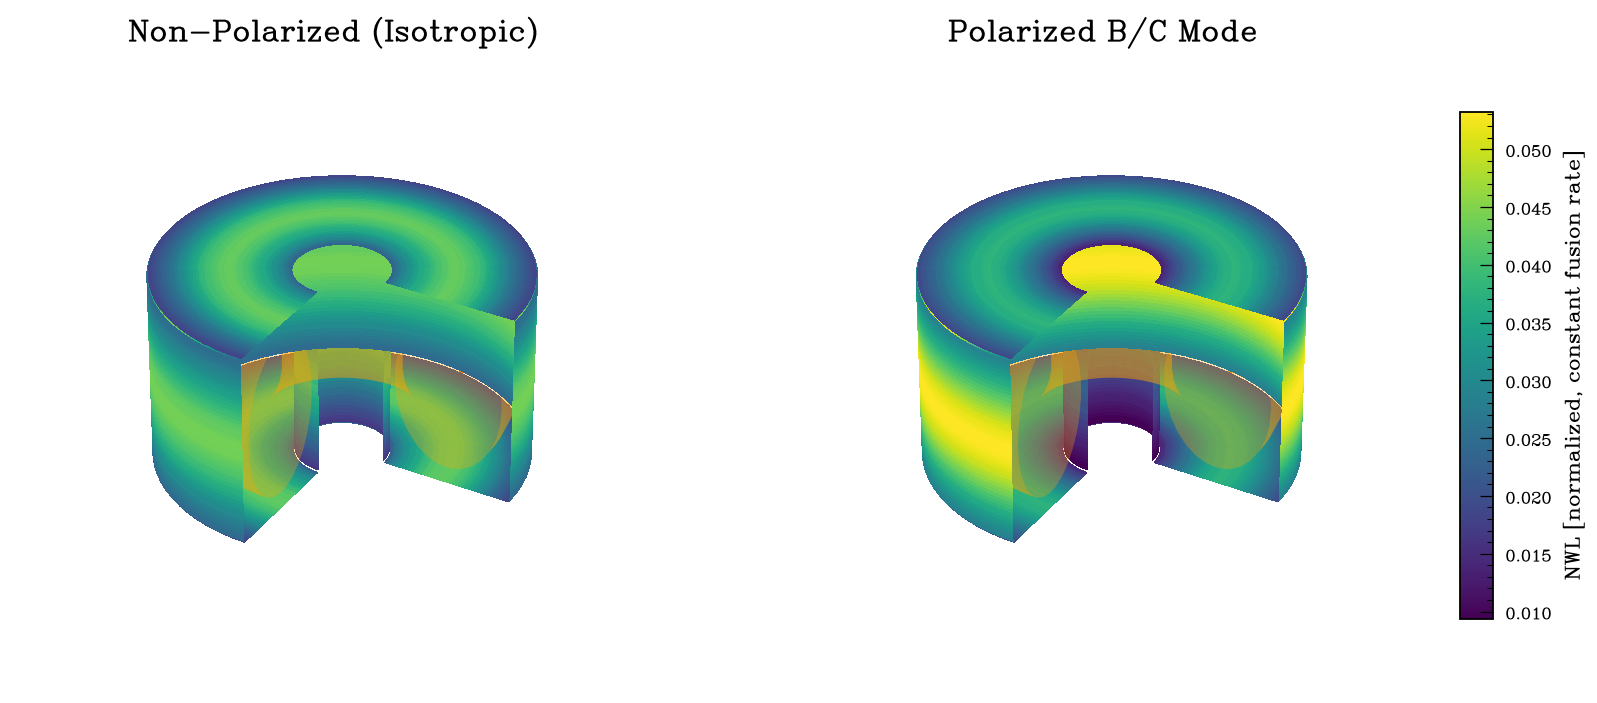
\includegraphics[width=0.82\linewidth]{tier3_torus3d.png}
  \end{center}
  \footnotesize \alert{Schematic} box-torus render of the computed free-streaming NWL (not CAD/DAGMC). Shared colorbar. Right (B/C) clearly \alert{darkens the center stack} and brightens the outboard wall vs the uniform isotropic case (left). Orange = schematic plasma source.
\end{frame}

% ======================================================================
\section{Part V --- Scope, limitations, and what's next}
% ======================================================================
\begin{frame}{What this model is --- and is not}
  \begin{itemize}
    \item \alert{Geometric, free-streaming NWL} (scattering OFF) --- \alert{not} a shielded dose, \alert{not} a TBR.
    \item \alert{Purely toroidal} field only (the angled-field \S3.2 kernels are not exercised).
    \item \alert{Filamentary / parabolic-ring} source; polarization $(a,b,c)$ a \alert{uniform} input (no depolarization).
    \item \alert{Single energy} (14.1 MeV); \alert{neutron channel only} (no alphas).
    \item \alert{Convex rectangular} cross section (no D-shape, no divertor, no occlusion).
  \end{itemize}
  \vfill
  The current ``inboard vs outboard'' fractions are a \alert{geometric precursor} to a TBR argument --- a real TBR needs a breeder blanket + scattering.
\end{frame}

\begin{frame}{Where does this sit in the literature?}
  \begin{itemize}
    \item The \alert{physics} is old (Kulsrud 1982); the \alert{analytic NWL} is Schwartz 2025 --- explicitly \emph{free-streaming}, positioned as the fast alternative to Monte-Carlo.
    \item Mainstream fusion-neutronics MC (ARC, ITER) uses \alert{isotropic} sources --- not a spin-polarization angular distribution tied to local $\Bhat$.
    \item A \alert{Monte-Carlo transport} implementation of the polarized emission appears \alert{open} (verify with domain experts; a search is not exhaustive).
  \end{itemize}
  \vfill
  So the reproduction \alert{validates the machinery}; the novel results come from the steps the analytic \emph{cannot} reach.
\end{frame}

\begin{frame}{Next steps (ranked, cost-honest)}
  \begin{enumerate}
    \item \alert{Angled / spatially-varying $\Bhat$} (cheapest). The sampler already rotates for any $\Bhat$; \texttt{anarr\'ima} has the angled kernels. \alert{The bridge to a physics-informed equilibrium source.}
    \item \alert{Scattering ON, real first wall} (moderate). The first result OpenMC gives that the analytic \emph{structurally cannot} --- the first honest step toward \alert{dose}. Loses the analytic ground truth $\Rightarrow$ new verification strategy.
    \item \alert{Breeder blanket $\to$ TBR} (new physics tier). Li enrichment, multiplier, tritium-production tallies. Highest effort, highest payoff.
  \end{enumerate}
\end{frame}

\begin{frame}{Summary}
  \begin{itemize}
    \item Spin polarization steers DT neutrons via $d\sigma/d\Omega(\theta\text{ to }\Bhat)$; A peaks $\perp$, B/C peak $\parallel$ (B$\equiv$C).
    \item Schwartz turns this into a fast, differentiable, \alert{free-streaming} analytic wall load.
    \item We built a \alert{validated} OpenMC polarization source: sampler ($6\times10^{-16}$ parity) $\to$ independent analytic ($\sim\!10^{-8}$ vs \texttt{anarr\'ima}) $\to$ full MC (residuals $\sim N(0,1)$).
    \item Honest engineering read: polarization \alert{redistributes} load (center-stack relief), and \alert{raises} peaking in a fixed geometry.
    \item The transport-capable source is the launchpad for scattering, blankets, and integration with a real plasma source.
  \end{itemize}
  \vfill
  \centering \footnotesize Reference: Schwartz, arXiv:2507.11758 (2025). \quad Code: \texttt{spf\_prototype/}.
\end{frame}

\begin{frame}[plain]
  \centering
  \vfill
  {\Large Thank you}\\[4pt]
  \small Questions, derivations, and the full \texttt{RESULTS\_tier\{1,2a,2b,3\}.md} are in \texttt{spf\_prototype/}.
  \vfill
\end{frame}

\end{document}
